% Author: Adolfo Centeno 
% Kubeet Corp
% www.kubeet.com

 
\documentclass{beamer}
\setbeamertemplate{navigation symbols}{}
\usepackage[utf8]{inputenc}
\usepackage{beamerthemeshadow}
\usepackage{listings}

\begin{document}
\title{Integration testing - Developer 3 - user Component}  
\author{Adolfo Centeno}
\date{\today} 

\begin{frame}
\titlepage
\end{frame}

\begin{frame}\frametitle{Table of contents}\tableofcontents
\end{frame} 


\section{install Angular - Integration Testing} 

\begin{frame}\frametitle{} 


\begin{block}{open new terminal, install Angular}
sudo npm install -g @angular/cli
\end{block}

\end{frame}


\begin{frame}\frametitle{} 

\begin{block}{fork repo}
\url{https://github.com/your-lider/angular-integration-testing.git} \\
click in fork
\end{block}

\begin{center}
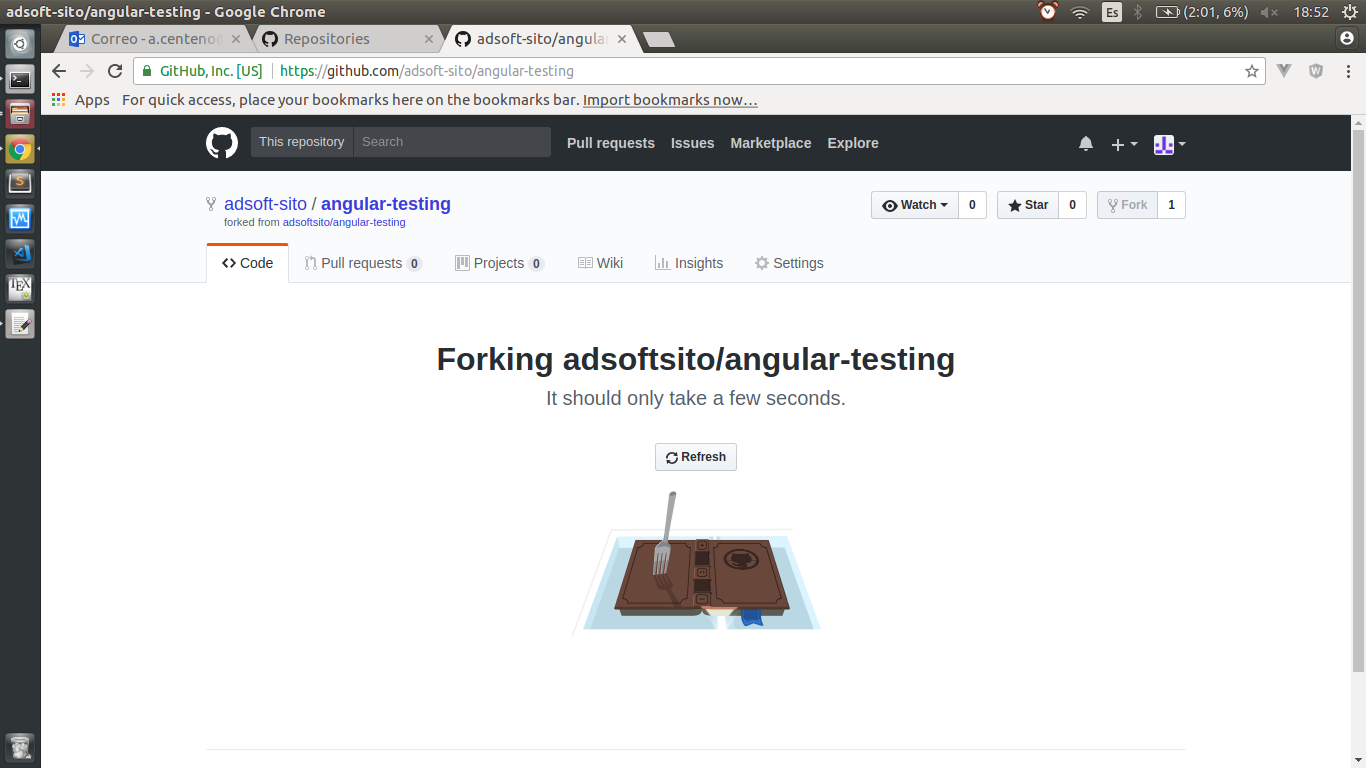
\includegraphics[width=0.9\textwidth]{forking.png}
\end{center}

\end{frame}




\begin{frame}\frametitle{} 

\begin{block}{clone your repo}
mkdir dev-integration-testing \\
cd dev-integration-testing	 \\
git clone -b develop https://github.com/your-own-repo/angular-integration-testing.git \\
cd angular-integration-testing \\
npm install \\
ng test   
\end{block}

\end{frame}


\begin{frame}\frametitle{} 

\begin{block}{user branch}
git branch \\
git branch user \\
git checkout user \\
git merge develop user \\
git branch 
\end{block}

\end{frame}


\begin{frame}\frametitle{} 

\begin{block}{create user, user-detail component}

ng generate component users \\
ng generate component user-details \\


\end{block}

\end{frame}



\begin{frame}\frametitle{} 

cd src/app/ \\


\begin{enumerate}
\item create : app.routes.spec.ts
\item update : app.routes.ts
\end{enumerate}


\end{frame}



\begin{frame}\frametitle{} 


cd src/app/user-details \\


\begin{enumerate}
\item update html and css files
\item update user-details.component.ts 
\item update integration test :  user-details.component.spec.ts
\end{enumerate}


\end{frame}


\begin{frame}\frametitle{} 


\begin{block}{push user branch}
cd .. \\
cd .. \\
pwd  \\
git add src/app/app.routes.ts \\
git add src/app/app.routes.spec.ts \\
git add src/app/user-details \\
git commit -m "user feature" \\
git push -u origin user \\
\end{block}
\end{frame}



\begin{frame}\frametitle{} 

\begin{block}{Go to github}
\url{https://github.com/} \\

create a pull-request to develop branch in lider repo
\end{block}

\begin{center}
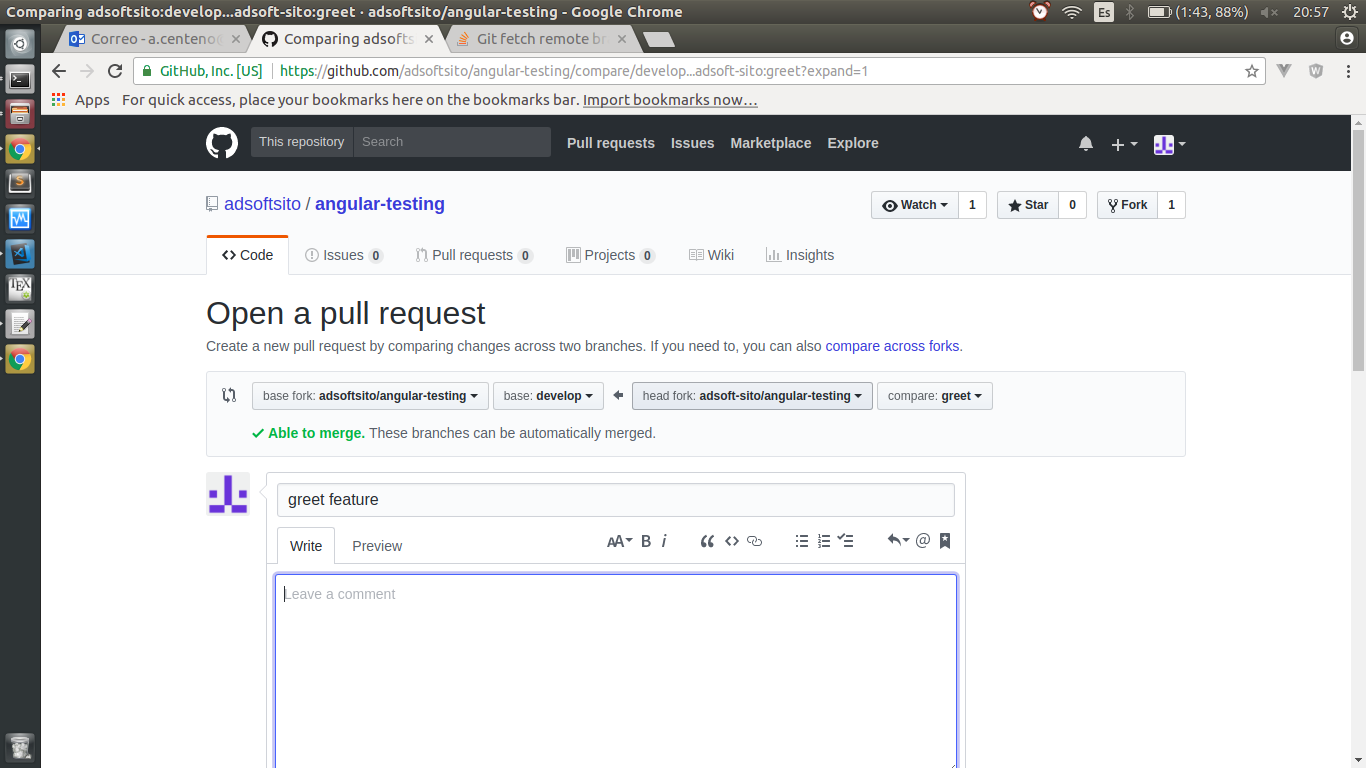
\includegraphics[width=0.9\textwidth]{pull-request.png}
\end{center}


\end{frame}


\end{document}
